\chapter{System Analysis}
\label{chap:chapter3}

In this chapter, it will be analysed the most relevant parts of the Testbed related with this project. A comparative study will be done in order to select the best option for each part, as much to electronics as to mechanical design. That chapter will be essential to have a proper design, presented in chapter \ref{chap:chapter4}.

The first part that will be studied is the Testbed Technology, in order to choose the best mechanical design for the air-bearing. Later, the electronics parts will be analysed and finnally some issues for the mechanical part, and a resumme of the communication system.

\section{ADCS Testbed Technology}\label{sec:Testbed}

Nowadays, the Testbed technology are in a constant growth. The need to have a low-friction environment, in order to simulate the aerospace environment, is the first condition that the Testbed has to fulfill. With that condition, the subsystems mounted in it, will be tested with a high precision, even with the constraint of the gravity that we have in the Earth. That is why the simulation of that kind of circumstances is not trivial. 

There are different types of simulations to achieve the torque-free environment, to have a friction-less ambience simulating the aerospace conditions. 

The first method consist of dipping the satellite or its subsystems into a tank of water. The first problem that appears with this method, is the covering that the satellite has to have to ensure that the water does not enter into the system, and because of that encapsulation, the gases generated inside the experiment does not get away.

Another method, but not too common, is the use of drop towers. For that manner of working, you will need a soft net (in some cases a solid like sand) in the end of the tower, to avoid that the satellite being damaged. Moreover, some high-speed cameras are used to take pictures while the satellite is descending, in order to analyse the attitude control. \cite{typestestbed}
Sometimes, that drop towers are used with the intent to create microgravity(see Figure \ref{fig:towernasa}). \cite{nasatower} 
 
\begin{figure}[H]
	\centering
		\includegraphics[scale=0.5]{capitulo2/towernasa.jpg}
	\caption{Drop Tower NASA \cite{nasatower}}
	\label{fig:towernasa}
\end{figure}

The third method, and the most common in the aerospace field, is the use of an air-bearing to create that low-friction atmosphere. That solution can not create a no-gravity environment, but it has a nearly free torque condition. The function of that air-bearing is to eject air under pressure through some small holes placed on a surface, normally spherical, to generate an air layer between the air-bearing and the rotor of the testbed platform.
There are two main types of Testbed for the satellites: Planar Air-Bearings and Spherical Air-Bearings. 

\begin{itemize}
\item \textbf{Planar Air-Bearings}. //
One of the most important characteristics of a Testbed, is the degrees of freedom (\acrshort{DOF}) that the air-bearing have. Planar Air-Bearing could have one or two \acrshort{DOF}(only \textbf{translational} type). 
For that case of air-bearing, the body that are being tested, carry its own cushion of air hovering upong a polished surface \cite{typestestbed}.

An example of that kind of air-bearing is in the Standford University's Aerospace Robotics Laboratory (ARL), used for the test of robotics for on-orbit construction (see Figure \ref{fig:ARL}). The experiment consist of two-link manipulator with two mini arms mounted at its end-point \cite{ARLtext}. 

\begin{figure}[H]
	\centering
		\includegraphics[scale=0.8]{capitulo2/ARL.jpg}
	\caption{ARL Testbed (planar air-bearing)\cite{ARLtext}}
	\label{fig:ARL}
\end{figure}

\item \textbf{Spherical Air-Bearings}. // Spherical air-bearings operate rotating a spherical or semispherical object above a convave structure using compressed air or gas, and perfectly matching with the sphere or semisphere.
In contrast to the planar air-bearings, which have translational \acrshort{DOF}, the shperical air-bearings have three  \textbf{rotational} \acrshort{DOF}. 

The angular constraint of the testbed depends on the size, shape and type of air-bearing. The three different types of spherical air-bearing are Dumbbell, Tabletop and Umbrella (see figure \ref{fig:airtypes}). 

\begin{figure}[H]
\centering
\subfloat[Dumbbell]{\label{fig:dumbbell} \includegraphics[width=70mm]{capitulo2/dumbbell.png}} 
\subfloat[Tabletop]{\label{fig:tabletop} \includegraphics[width=70mm]{capitulo2/tabletop.png}} \\
\subfloat[Umbrella]{\label{fig:umbrella} \includegraphics[width=70mm]{capitulo2/umbrella.png}} 
\caption{Spherical Air-Bearings Styles \cite{typestestbed}} \label{fig:airtypes}
\end{figure}

The description and some examples of each one is presented below:
\begin{itemize}
\item \textit{Dumbbell}. That type of air-bearing offset the \acrshort{COR} and extend two arms, one per side. Dumbbell testbed allow the 360º of freedom in the yaw and roll axes (see figure \ref{fig:dumbbell}). An example of that style of Testbed is shown in figure \ref{fig:exampledumbbell}, an air-bearing of the University of Michigan known as the Triaxial Attitude Control Testbed (\acrshort{TACT}). In that figure, you can see the different actuators that the \acrshort{TACT} has: reaction wheels, fans and mass actuators. \cite{michigantestbed}

\begin{figure}[H]
	\centering
		\includegraphics[scale=0.8]{capitulo2/exampledumbbell.jpg}
	\caption{TACT Dumbbell Style air-bearing \cite{michigantestbed}}
	\label{fig:exampledumbbell}
\end{figure}

\item \textit{Tabletop}. In this testbed, the table where the different subsystems are located, is mounted above a semisphere directly. Whith that type of air-bearing is allowed the 360º motion in the yaw axis (see figure \ref{fig:tabletop}), but a limited motion in the pitch and roll axes. The advantages of this solution are the inexpensive fabrication that it has and the little space that it requires. Virginia Polytechnic Institute & State University have built a satellite \acrshort{ADCS} testbed with the use of two spherical air-bearings: a tabletop style in each side of a dubbell air-bearing \cite{virginia}. Figure \ref{fig:tabledumd} shows the tabletop
air-bearing with the dumbbell part of the air-bearing base in the background of the photo.

\begin{figure}[H]
	\centering
		\includegraphics[scale=0.8]{capitulo2/tabletopanddumbbell.jpg}
	\caption{DSACSS Air-Bearing Set \cite{virginia}}
	\label{fig:tabledumd}
\end{figure}

\item \textit{Umbrella}. The last type of spherical air-bearing is an improvement of tabletop. In order to have a better freedom motion in axes pitch and roll, a rod from a fully spherical bearing is placed, permitting more \scrshort{DOF}. As tabletop testbed, it has a 360º of freedom in the yaw axis, and a bigger table can be mounted on it, without the loss of freedom motion (see figure \ref{fig:umbrella}).\ref{fig:airtypes}
\end{itemize}
\end{itemize}

The \gls{GranaSAT} testbed will be designed as a improvement of tabletop system. Rather than have the subsystems in a table outside of the semisphere, we have include the subsystems inside of the semisphere, in order to have more \acrshort{DOF} in axes pitch and roll, and less weight discarding the table that tabletop or umbrella have (see figures \ref{fig:umbrella} and \ref{fig:tabletop}). The design of that testbed will be fully covered in the next chapter.  


\section{Sensors for the \acrshort{ADCS}}\label{sec:sensors}

In order to take measures of the actual state of the system, some sensors should be used in the \acrshort{ADCS} (see figures \ref{fig:ADCS2} and \ref{fig:ADCS}, where a diagram of that kind of systems is represented). 

\acrshort{ADCS} will use different ways of measurements to acquire the attitude of the system, depending of the kind of sensors, that attitude will be relative or absolute, but the most used are the relative sensors, which use external references to orientate the whole system.

Some of the most common references used by the satellites are from the Sun, stars, Earth's horizon, Earth's Magnetic field, and some inertial measurements as for example the angular velocity of the satellite, in order to obtain the attitude when the external references are not available.

\begin{itemize}

\item \textbf{Star Sensor}. Also known Star tracker, is an optical device (photocells or a camera) that measures the position of a star group from the sky. The star tracker uses a pattern recognition of the star constellations in the Field of view (\acrshort{FOV}) and by means of a star catalogue covering the whole firmament. The orientation of the satellite can be determined finding that pattern by comparing the optical detection (for example an image) with that catalogue. That reference is one of the most accurate (see table \ref{tab:comparisonsensor}) because they use the fixed stars. The figure \ref{fig:startracker}  shows the diagram and a photo of a commercial star tracker. 
\begin{figure}[H]
\centering
\subfloat[Star tracker diagram \cite{manu}]{\label{fig:startracker1} \includegraphics[width=90mm]{capitulo3/startracker.jpg}}
\subfloat[Commercial Star Tracker - CT-633 \cite{ballaerospace}]{\label{fig:startracker2} \includegraphics[width=50mm]{capitulo3/startracker2.jpg}}
\caption{Star tracker} \label{fig:startracker}
\end{figure}

Because of its dimensions(in some cases) and the need of a big quantity of data for the catalogue, that kind of sensor is not very common in Cubesats.
\item \textbf{Horizon Sensor}. That kind of sensor measures the difference between the darkness of space and the light bouncing of the Earth. In other words, finds the Earth’s horizon thus the orientation relatively to the blue planet. Its problem is the low accuracy. Now in the table \ref{tab:comparisonsensor} there will be a better comparison with the other sensors, where that affirmation will be confirmed.

Depending on the kind of the horizon sensor, it uses an infrared diode and a lens or a camera, and it can be a scanner or horizon crossing indicators.  Due to size, weight and complexity the last one are considered the most suitable for the CubeSat. Moreover, for the satellites, it has to be used together with other attitude sensors.

The figure \ref{fig:horizonbexus} shows a capture of the \acrshort{GS} representing the horizon sensor measurements of the GranaSAT BEXUS Team.

\begin{figure}[H]
	\centering
		\includegraphics[scale=0.8]{capitulo3/horizon.jpg}
	\caption{Horizon Sensor scheme \cite{carlos}}
	\label{fig:horizon}
\end{figure}

\begin{figure}[H]
	\centering
		\includegraphics[scale=0.75]{capitulo3/horizonbexus.jpg}
	\caption{Horizon Sensor GranaSAT BEXUS \cite{Gsat}}
	\label{fig:horizonbexus}
\end{figure}

\item \textbf{Sun sensor}. The Sun sensor is used for providing a vector measurement of the Sun radiation using photodiodes, photoresistors, solar cells etc.
The most relevant problem that the sun sensor has is they need direct sunlight and the solar cells should be replaced by the sun sensors(less power for the satellite). The other problem is the need of the sun, because when the sun is hidden, that sensor has no functionality (see figure \ref{fig:shadow}). Similarly, the same problem but with the opposite case, a reflective surface can damage the measurements(see figure \ref{fig:light}). It can be analog or digital, but the most accurate is the second one \cite{sunsensor}.
The analog one works depending on the angle and the current flow, this is why is not accurate (1º of accuracy in \acrshort{FOV} of 30º).

\begin{figure}[H]
	\centering
		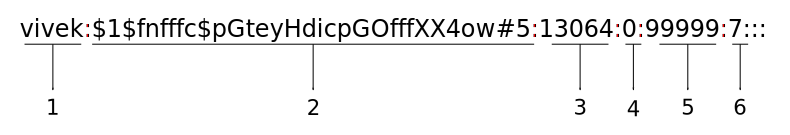
\includegraphics[scale=0.8]{capitulo3/shadow.jpg}
	\caption{Possible shadow of a larger satellite \cite{sunsensor}}
	\label{fig:shadow}
\end{figure}


\begin{figure}[H]
	\centering
		\includegraphics[scale=0.8]{capitulo3/light.jpg}
	\caption{Possible reflection in the sun sensor \cite{sunsensor}}
	\label{fig:light}
\end{figure}

\item \textbf{Magnetometer}. It is a sensor which measures the Earth's field. In Low Earth Orbit \acrshort{LEO}, where the magnetic field of the Earth is the sufficient strong and \acrshort{3D} magnetometer will provide a proper attitude determination. there are three types: fluxgate, magneto-resistive and magneto-inductive. They should be well calibrated in order to have the control about the field generated within the Cubesat, in that case, Testbed. If the sensor is perfectly calibrated, that option is one of the best because of its good accuracy. The measurements are compared with a model of the Earth's magnetic field (database). They will be really useful because of the use of magnetorquers in our project. (see sectionNCNCNCFJDJDN)

\item \textbf{Accelerometer}. It is a inertial sensor, and measure translatory accelerations. The \acrshort{MEMS}  inertial accelerometers consists of a mass-spring system in a vacuum. When it is exercised an acceleration on the sensor, the mass in the spring system is displaced. The description of that functionality is shown in the figure \ref{fig:accelerometer}, a sensor capacitive with \acrshort{MEMS} technology. When the mass is moved of its original position, the capacitance changes and, then, the voltage too.

\begin{figure}[H]
	\centering
		\includegraphics[scale=0.8]{capitulo3/accelerometer.jpg}
	\caption{\acrshort{MEMS} accelerometer\cite{accelerometer}}
	\label{fig:accelerometer}
\end{figure}


\item \textbf{Gyroscope}. That kind of sensor will measure the angular velocity of the body about a specified axis of rotation, in this case the Testbed, without the need of a external reference.
The detumbling phase that sensor would be really relevant.
The detumbling phase is produced when the satellite is launched from the rocket and it starts to travel around the orbit. In that moment, the Cubesat starts to turn on itself with a high angular velocity, so the objective of that phase is to stop that turn, stabilize it, in order to take a proper attitude determination. The stabilization is made thank to the actuators of the system. But in our case, the Testbed will have a manual rotation in order to simulate that situation.
The figure \ref{fig:gyros} shows how a \acrshort{MEMS} gyroscope can be modeled in a easy way.

\begin{figure}[H]
	\centering
		\includegraphics[scale=0.8]{capitulo3/gyros.jpg}
	\caption{\acrshort{MEMS} gyroscope\cite{gyros}}
	\label{fig:gyros}
\end{figure}

\end{itemize}

Now it is time to get a comparison table  of the sensors described above(table \ref{tab:comparisonsensor}), in order to select the best option for our system.
 
\begin{table}[H]
\centering
\begin{tabular}{|l|l|l|l|}
\hline\hline
\textbf{Type}		 				 & \textbf{Initial attitude acquisition}	& \textbf{\acrshort{DOF}} & \textbf{Accuracy}			\\	\hline
Magnetometer						 & Yes																		& 3												&		1 arcminute										\\ 	\hline
Radio Frequency beacon   & Yes  																	& 2												& 	1 arcminute										\\ 	\hline
Horizon sensor   				 & Yes 																		& 2 											&   5 arcminutes  								 	\\ 	\hline
Sun sensor    					 & Yes 																		& 2												&   1 arcminute									\\ 	\hline
Solar panel   					 & Yes 																		& 2 											&   1º										\\	\hline
Star tracker    				 & Yes 																		& 3  											&  	1 arcsecond								\\	\hline\hline
\end{tabular}
\caption{Comparison of some kind of sensors \cite{liebe}}\label{tab:comparisonsensor}
\end{table}

Because of the Cubesat limitations in size and weight, the sensors chosen are the magnetometer, accelerometer and gyroscope. Each sensor will be used in \acrshort{MEMS} technology, in order to have the smallest size possible. Because the studied design for the Testbed, maybe it will be used for the Cubesat if it is possible.

\textbf{Gyroscope Choice}
The following table \ref{tab:gyroscope} presents the comparison of three different \acrshort{3D} gyroscopes MEMS technology, but for the Testbed, it will be used the \textbf{test board} of each one, in order to be used it in the breadboard for the simulations and tests, and to have an easier soldering process. However, the future cubesat will have only the chip sensor.

\begin{table}[H]
\centering
\begin{tabular}{|l|l|l|l|}
\hline\hline
\textbf{Parameter}		 				 & \textbf{L3G4200D}	& \textbf{MPU6050} & \textbf{L3GD20H}			\\	\hline
Accelerometer incorporated		 & No													& Yes												&		 No										\\ 	\hline
Voltage Supply\footnote{Voltage supply for the test board}(V) &  			5														& 5												& 	 5										\\ 	\hline
 Temperature range (ºC) 	 & -40 to 85						& -40 to 85										&  -40 to 85  								 	\\ 	\hline
Scale range (º/sec)   			&\begin{equation*}  \left\lbrace  \begin{array}{l}     \pm250 \\     \pm500 \\\pm2000\\ \end{array}  \right.\end{equation*}  &
\begin{equation*}  \left\lbrace  \begin{array}{l}     \pm250 \\     \pm500 \\\pm1000 \\\pm2000\\ \end{array}  \right.\end{equation*}  &   
\begin{equation*}  \left\lbrace  \begin{array}{l}     \pm245 \\     \pm500 \\\pm2000\\ \end{array}  \right.\end{equation*}								\\ 	\hline
Sensitivity (mdps/digit)	 & 	8.75,  17.50,  70		& 7.6, 15.2, 30.4, 60.8 &  8.75,  17.50, 70.00								\\	\hline
Output data rate (Hz)  & 100-800	& 4-8000		& 11.9-757.6		\\	\hline
Communication protocol  & I2C											& I2C		&  I2C							\\	\hline
Consumption at 3.3V (mA)  & 6.1											& 3.9	& 	5				\\	\hline
\hline
\end{tabular}
\caption{Comparison of gyroscopes \cite{MPU6050}\cite{L3G4200D}\cite{L3GD20H}}\label{tab:gyroscope}
\end{table}

In conclusion, the best option is MPU6050. The features that have not been compared are practically the same values. Moreover, that sensor includes an accelerometer, so it will no be necessary includes one more sensor for the accelerometer. In chapter \ref{chap:chapter4}, section \ref{sssec:GyrAc} MPU6050 will be explained in more detail.

For the magnetometer, see the project of the magnetic part for the Testbed \cite{alejandro}.

\section{\acrshort{ADCS} Actuators}\label{sec:actuators}

To control the position of the Testbed, the \acrshort{ADCS} generates torques thanks to the actuators. There are two kinds of actuators:
\begin{itemize}
\item Passive actuators. That kind of actuator does not require power or fuel, however, it can restrict control over the spacecraft’s attitude. For that reason, it is not commonly used. For example: 
\begin{itemize}
\item Permanent magnets. They are passive electromagnets  and can only align a satellite axis in one orientation relative to the Earth's magnetic field. That kind of actuator is permanent, so, for that reason, they normally are paired with other one. 
\item Hysteresis rods. The Earth's magnetic field magnetizes the rods and they uses the hysteresis effect working against the spinning motion. See figure \ref{fig:rods} where is represented that kind of actuator in a Cubesat and the permanent magnets too.
\begin{figure}[H]
	\centering
		\includegraphics[scale=0.8]{capitulo3/rods.jpg}
	\caption{Permanent magnets and Hysteresis rods actuators - GeneSat-1 \cite{genesat}}
	\label{fig:rods}
\end{figure}

\item Gravity gradient boom. That boom as a mass at the end of the boom which will be aligned with the center of the Earth.
\end{itemize}
\item Active actuators. The opposite kind, active actuators requires fuel or energy to control, but in this case, the control is greater than passive types. For example: magnetorquers, reaction wheels and thrusters. The last one is not really used because of its fuel consumption, which add weight to the Cubesat and it is not recommendable. That type will be explained in more detail below.
\end{itemize}

For the Testbed, the group chosen is the active actuators, because they have a great control of the attitude. Now, inside this group, the thrusters is discarded, because it will need a determined quantity fuel to control them. Then, for the Testbed, the best two options are the reaction wheels and the magnetorquers, which will be described and we will choose the best materials and options for the Testbed application. In this project, the only actuator which will be studied is the reaction wheels, because the magnetorquers will be studied in the project where the magnetic part for the Testbed is treated \cite{alejandro}.

\textbf{Reaction wheels}. Belongs to the active group and they are radial weights that are spun with the use of electric motors. The reaction wheel, will change the Testbed (or Cubesat) angular velocity, changing the angular velocity of the reaction wheel in the opposite direction. Normally there are three reaction wheels (aligned orthogonally), in order to have the control of the three dimensions. That actuator not interacts with external torques and it has a fast acting if the size is the correct. Because of the saturation problem, in order to decrease the stored momentum and required energy, other actuator is normally place with the reaction wheels, in our case, the magnetorquers.

The material of the wheel is the first item that is going to be studied. The table \ref{tab:wheel} shows the different material that we have available to buy, because of its prize and the stock in different stores in Granada.

\begin{table}[H]
\centering
\begin{tabular}{|l|l|}
\hline\hline
\textbf{Material} & \textbf{Density ($Kg/m^3$} \\ \hline\hline
Copper            &8940   \\ \hline
Bronze             & 8890\\ \hline
Iron         & 7870\\ \hline
Aluminium         & 2700\\ \hline\hline
\end{tabular}
\caption{Different materials for the wheel} \label{tab:wheel}
\end{table}

The best options depending on the density of the material are the copper and bronze, but finally the choice was \textbf{bronze} because of the availability in the diameter needed after of the calculation shown in section \ref{ssec:reactionwheels}. The figure \ref{fig:bronze} shows the bronze bar bought. When the reaction wheels were manufactured, the outer surface was cleaned (see figure \ref{fig:bronze2}), anyway, in chapter \ref{chap:chapter5} that process will be described.

\begin{figure}[H]
	\centering
		\includegraphics[scale=0.8]{capitulo3/bronze.jpg}
	\caption{Bronze bar for the reaction wheels}
	\label{fig:bronze}
\end{figure}


\begin{figure}[H]
	\centering
		\includegraphics[scale=0.1]{capitulo3/bronze2.jpg}
	\caption{Manufactured wheel}
	\label{fig:bronze2}
\end{figure}


The next step is the selection of the motors for the wheels.  Because of their sizes and the availability in the laboratory, we used \acrshort{DC} Motors from \acrshort{CD} players of the recycled \acrshort{PC}s available in the Project's Laboratory of the \acrshort{ECTD}, so the cost of that motors were zero.

Now, in the table \ref{tab:motors} there will be a comparison of the motors found on that \acrshort{CD} players.

\begin{flushleft}
\begin{table}[H]
\begin{tabular}{ | l | l | l | l | l | l | }
\hline\hline
	\textbf{Parameter} & \textbf{Minebea} & \textbf{Mitsumi} & \textbf{Kysan} & \textbf{Kysan} & \textbf{Mabuchi} \\ \hline
	\textbf{Model} & MDN3BT& M25E-4 & RF-300CH & RF-300CA & RF-300C \\ \hline
	\textbf{Voltage range (V)} & 0.7-6.0 & 1.0-7.0 & 1.0-6.3 & 0.7-5.0 & 1.5-6.0 \\ \hline
	\textbf{Rated Voltage (V) }& 2 & 5 & 3 & 2 & 3 \\ \hline
	\textbf{No load speed (RPM)} & 2305 & * & 3000 & 2200 & 3500 \\ \hline
	\textbf{No load current (mA)} & 16 & * & 18 & 18 & 22 \\ \hline
	\textbf{Torque (mN-m)} & 0.392 & 1.47 & 0.42 & 0.27 & 0.48 \\ \hline
	\textbf{Speed at torque (RPM)} & 1458 & 2750 & 2400 & 1600 & 2830 \\ \hline
	\textbf{Current  at torque (mA)} & 71 & 300 & 65 & 55 & 93 \\ \hline\hline
\end{tabular}
\caption{Comparison of motors \cite{Minebea}\cite{Kysan}\cite{Mitsumi}\cite{Mabuchi}}\label{tab:motors}
\end{table}
\end{flushleft}

Moreover, there where two more motors without name, model or brand, so they should be tested in order to take the characteristics. In chapter \ref{chap:chapter5} there will be a characterization of the motors, with and without the wheel. The characteristics described in table \ref{tab:motors} are practically similar, so we have to take in account other details: mechanical design, dimensions, connector, etc. And finally the chosen motors were Kysan (RF-300CH model), Minebea and one without name, because the connection and the sizes were the same, as described in figures \ref{fig:motorconnection} and \ref{fig:motorsize}.

\begin{figure}[H]
	\centering
		\includegraphics[scale=1.5]{capitulo3/motorconnection.jpg}
	\caption{Motor connection}
	\label{fig:motorconnection}
\end{figure}

\begin{figure}[H]
	\centering
		\includegraphics[scale=0.8]{capitulo3/motorsize.jpg}
	\caption{Motor dimensions \cite{Minebea}}
	\label{fig:motorsize}
\end{figure}

\section{On-board microprocessor selection}\label{sec:microprocessor}

In order to use the libraries provided by the sensors suppliers, we decided to use Arduino code, but instead of use a complete board of Arduino, the decision was take only the microprocessor AVR chip and the needed circuit components to work with it. Now, it is needed the selection of which microprocessor of Arduino is the best for our project, so the best way to select is comparing the main characteristics of some of them (see table \ref{tab:microprocessorcompare}).
\begin{table}[H]
\centering
\begin{tabular}{ | l | l | l | l | }
\hline\hline
	\textbf{Model} & \textbf{ATmega2560} & \textbf{ATmega8-16AU} & \textbf{ATmega328P-AU} \\ \hline\hline
	\textbf{SRAM (KB) }& 8 & 1 & 2 \\ \hline
	\textbf{ROM (KB)} & 256 & 8 & 32 \\ \hline
	\textbf{EEPROM (B)} & 4096 & 512 & 1024 \\ \hline
	\textbf{IO Pins} & 86 & 23 & 23 \\ \hline
	\textbf{Speed (MHz)} & 16 & 16 & 20 \\ \hline
	\textbf{ADC-Bits} & 10-bit & 10-bit & 10-bit \\ \hline
	\textbf{PWM} & 16 & 3 & 6 \\ \hline
	\textbf{Min Supply Volts (V)} & 1.8  & 2.7  & 1.8   \\ \hline
\textbf{	Timers Counters} & 6 & 3 & 3 \\ \hline
	\textbf{SPI} & 5 & 1 & 2 \\ \hline
	\textbf{TWI (I2C)} & 1 & 1 & 1 \\ \hline
	\textbf{UART} & 4 & 1 & 1 \\ \hline
	\textbf{ADC channels} & 16 & 8 & 8 \\ \hline
	\textbf{Ext Interrupts} & 32 & 2 & 24 \\ \hline
	\textbf{Price (€)} & 17,12 & 3,72 & 3,41  \\\hline\hline
\end{tabular}\caption{Comparison of microprocessors \cite{microprocessorcompare}}\label{tab:microprocessorcompare}
\end{table}

The best option for the Testbed project is the ATMEGA328P-AU, because it has the necessary analog and digital pins and it is the cheapest one. That microprocessor is used in \acrshort{THT} model in Arduino UNO, but we will use the \acrshort{SMD} model to save weight and space in the \acrshort{PCB}. In section \ref{sssec:micro} the microprocessor will be explained in more detail.


